\chapter{Marco Teórico}
\label{marcoteorico}

%Aquí va una lista:
%\begin{itemize}
    %\item Ingeniería Informática.
    %\item Ingeniería Sonido e Imagen en Telecomunicación.
    %\item Ingeniería Multimedia.
    %\begin{itemize}
         %\item Mención: Creación y ocio digital.
         %\item Mención: Gestión de Contenidos.
    %\end{itemize}
%\end{itemize}



\section{¿Que es un sitio Web?}


Un sitio web es un conjunto de documentos generados en HTML/XHTML relacionadas entre si y que pertenecen a un mismo dominio. Es sitio es accesible generalmente mediante el protocolo de comunicación HTTP(Hypertext Transfer Protocol). En estas páginas web, se componen principalmente de información, generalmente texto, hiperenlaces y multimedia. En función del contenido generado se pueden clasificar dos tipos de sitios web:

\begin{itemize}
  \item \textbf{Estáticos}: Los sitios web estáticos, muestran información permanente, creadas mediante HTML. Estos sitios no acceden a una base de datos para obtener el contenido. Normalmente estos sitios web e utilizan cuando el contenido no va a sufrir cambios en la información del sitio.
  \item \textbf{Dinámicos}: Los sitios web dinámicos, por el contrario si que acceden a una base de datos para acceder al contenido y reflejar los resultados en el sitio web. En los sitios web dinámicos, el administrador del sitio podrá agregar, modificar y eliminar el contenido mediante un gestor de contenidos. Para crear estos sitios se requiere uso de lenguajes de programación(como PHP).
\end{itemize}


Para que el sitio web sea visible para los buscadores, y por tanto más accesibles para los usuarios se utilizan técnicas de posicionamiento SEO

Un sitio web se ha convertido en una tarjeta de presentación digital, ya sea para empresas, organizaciones, o personas, así como una manera de comunicar ideas, pensamientos, conocimientos, informaciones o teorías. Así mismo, la nueva tendencia orienta a que las páginas web no sean sólo atractivas para los internautas, sino también optimizadas (preparadas), para los buscadores a través del código fuente. Forzar esta doble función puede, sin embargo, crear conflictos respecto de la calidad del contenido.


\section{Aplicación Web}

Una aplicación web application es un programa de software basado en la arquitectura cliente–servidor que un usuario ejecuta en un navegador. En la arquitectura cliente servidor se suelen distinguir tres niveles: el cliente, el servidor y la base de datos.


\subsection{Cliente} 
Es el nivel superior que interacciona con el usuario, solicita a un servidor Web el envio de los recursos mediante HTTP.La parte cliente de las aplicaciones web suele estar formada por el código HTML que forma la página web más algo de código ejecutable realizado en lenguaje de script del navegador (JavaScript).


\subsection{Servidor} 
El servidor web es un programa que está esperando permanentemente las solicitudes de conexión mediante el protocolo HTTP por parte de los clientes web. 
La parte servidor de las aplicaciones web está formada por:
Páginas estáticas (documentos HTML) que siempre muestran el mismo contenido.
Recursos adicionales que se pueden emplear dentro de las páginas o estar disponibles para ser descargados y ejecutados (visualizados) en el cliente.
Programas o scripts que son ejecutados por el servidor web cuando el navegador del cliente solicita algunas páginas. La salida de este script suele ser una página HTML estándar que se envía al navegador del cliente.




\section{Historia del Desarrollo Web}


\begin{figure}
\begin{center}
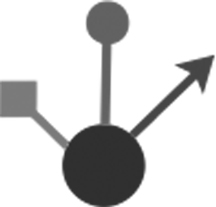
\includegraphics[scale=0.25]{imagenes/logoim.jpg}
\caption{Logo de Ingeniería  Multimedia.}
\label{logo_im}
\end{center}
\end{figure}

\begin{figure}
\begin{center}

\includegraphics[scale=0.25]{imagenes/logoeps.jpg}
\caption{Logo de la EPS.}
\label{logo_eps}
\end{center}
\end{figure}

\section{Desarrollo de Aplicación Web}


Por supuesto, puedes mejorar esta presentación utilizando mas modificadores. Esta información y mucha más puede ser encontrada en \cite{listing_packagge} y en \cite{heinz1listings}.

Otro ejemplo, ahora para mostrar código PHP, sería escribir en tu fichero \LaTeX lo siguiente:
\begin{verbatim}
 \begin{lstlisting}[style=PHP, caption={ejemplo código PHP},label=PHP_code]
 /* 
Ejemplo de código en PHP para escribir tu primer programa en este lenguaje
Copia este código en tu ordenador y ejecútalo
*/
<html>
  <head>
    <title>Prueba de PHP</title>
  </head>
  <body>
    <?php echo '<p>Hola Mundo</p>'; ?> //esto lo escribe TODO el mundo
  </body>
</html>
 \end{lstlisting}
\end{verbatim}
 
 y el resultado es: (ver listado \ref{PHP_code})
 
\section{Arquitecturas y Conceptos Básicos} 